\section{Results \& Discussion}\label{results}

% O =
%     4 0 4
% E =
%     739 131 50
%     589 690 92
%     302 571 664

In this section the obtained results are shown and discussed. First we present the results for the analysis of the system through the metrics and with only the local controller. In Figure~\ref{fig:closed_o000} and Figure~\ref{fig:open_o101}  we show two cases of the evolution of the three metrics after the startup of the system.

\begin{figure}[ht]
    \centering
    \begin{subfigure}[t]{0.32\textwidth}
    \centering
    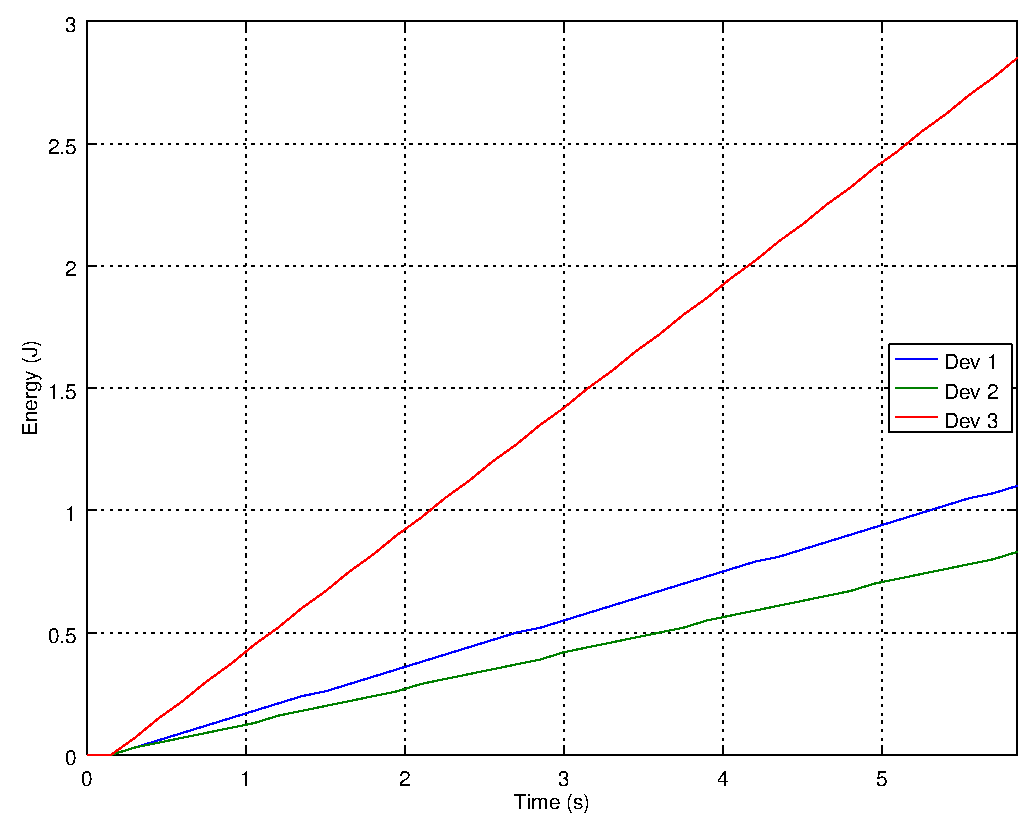
\includegraphics[width=.95\textwidth]{img/e_closed_o000}
    \caption{Energy over time of the 3 luminaires.}
    \label{fig:e_closed_o000}
    \end{subfigure}
    \begin{subfigure}[t]{0.32\textwidth}
    \centering
    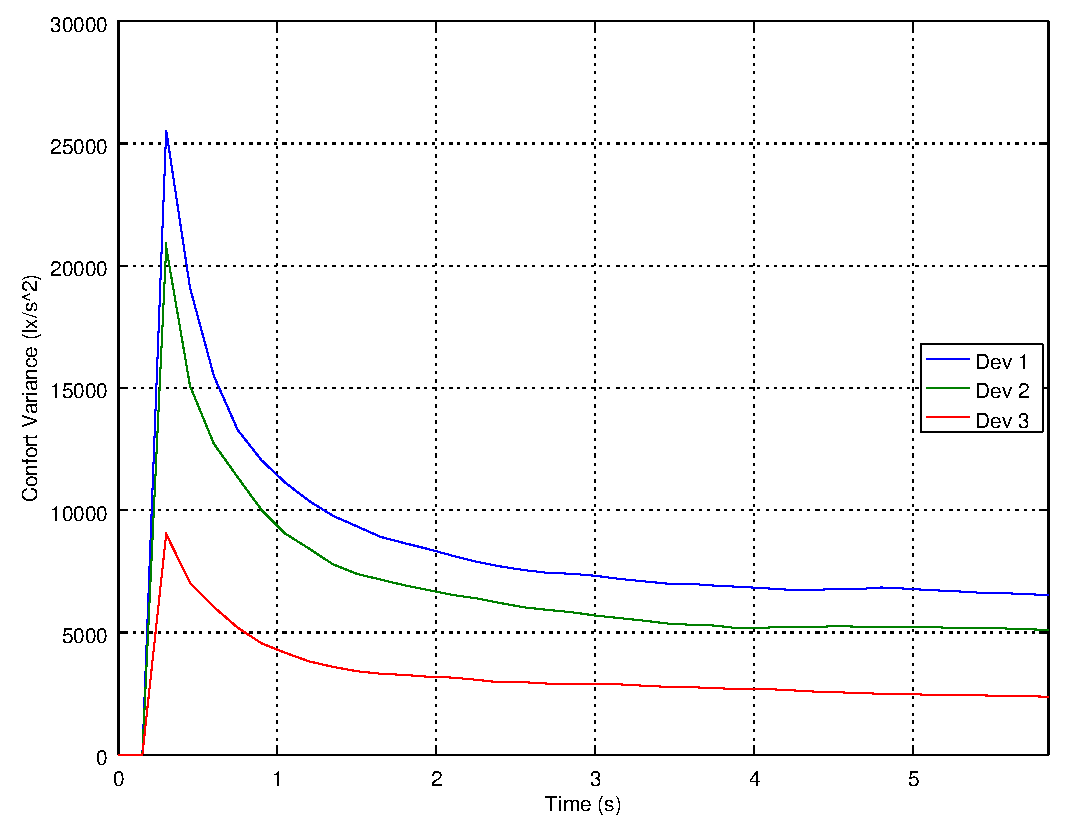
\includegraphics[width=.95\textwidth]{img/f_closed_o000}
    \caption{Comfort variance over time of the 3 luminaires.}
    \label{fig:f_closed_o000}
    \end{subfigure}
    \begin{subfigure}[t]{0.32\textwidth}
    \centering
    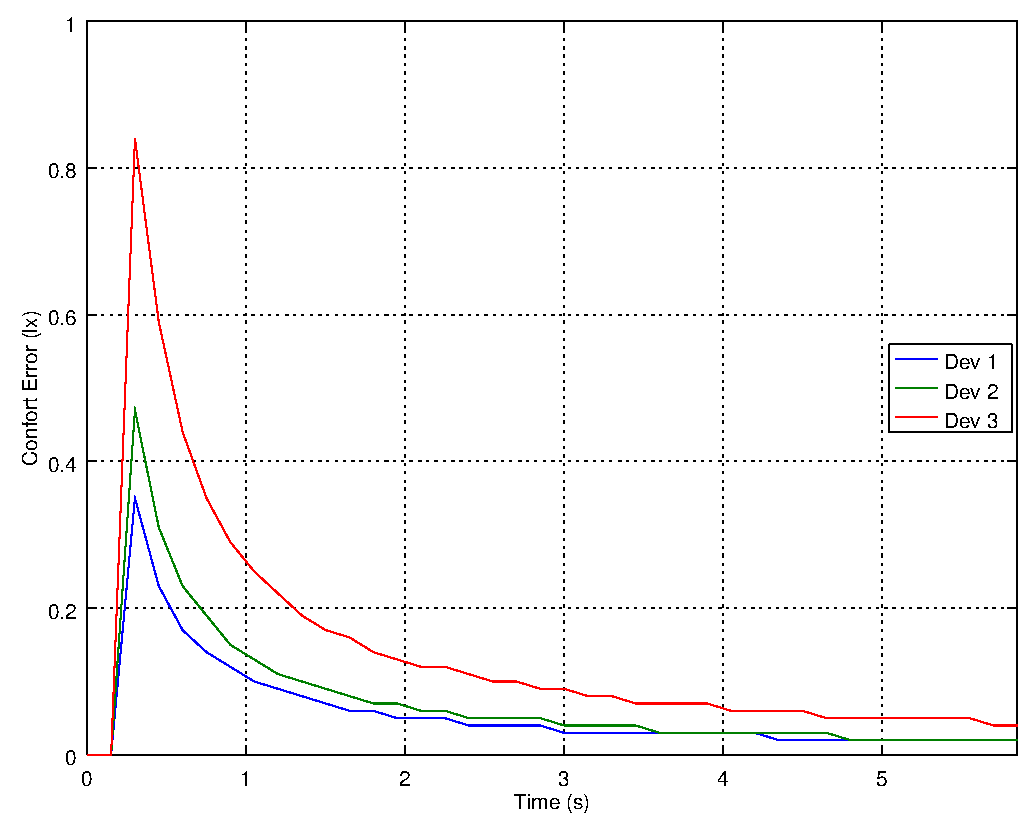
\includegraphics[width=.95\textwidth]{img/n_closed_o000}
    \caption{Comfort error over time of the 3 luminaires.}
    \label{fig:n_closed_o000}
    \end{subfigure}
    \caption{Metrics after system startup with the box closed and all desks as unoccupied. }
    \label{fig:closed_o000}
\end{figure}

The first figure corresponds to the system without external light and with all the references to the lower value 15 (unoccupied state). The energy spent rises in a linear way in all illuminaires, with desk 3 rising faster. This can be explained if we consider all luminaires to be at a fixed, but different, duty cycle, with luminaire 3 being the one with the LED at a higher intensity. Both the comfort error and the confort variance present the same behaviour, with the difference that the error tends to 0, while the variance tends to a small, but larger than 0, value. The initial spike in both metrics is explained by the startup of the Local controller, when all LED's are off. The remaining value in the variance shows that there is some flicker in the LED's that is however unnoticeable with a naked eye. This flicker can be explained by noise on the reading of the illuminance or due to not enough precision with the PWM or even some lack of tuning in the PID.

\begin{figure}[ht]
    \centering
    \begin{subfigure}[t]{0.32\textwidth}
    \centering
    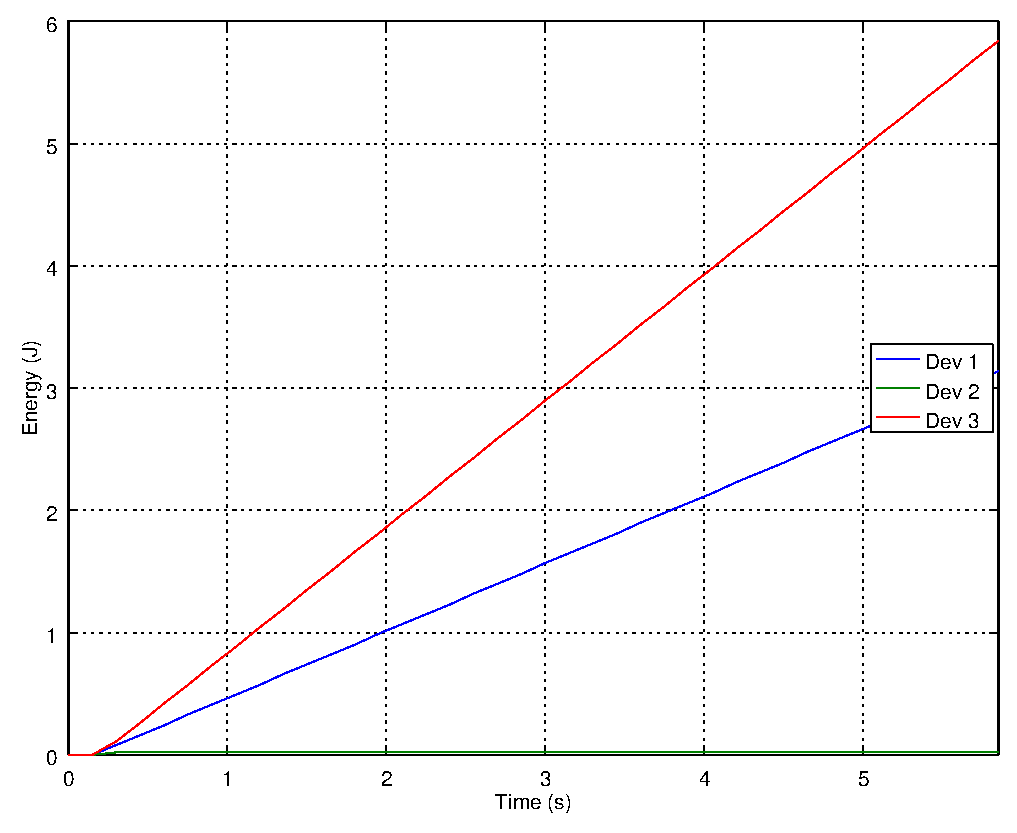
\includegraphics[width=.95\textwidth]{img/e_open_o101}
    \caption{Energy over time of the 3 luminaires.}
    \label{fig:e_open_o101}
    \end{subfigure}
    \begin{subfigure}[t]{0.32\textwidth}
    \centering
    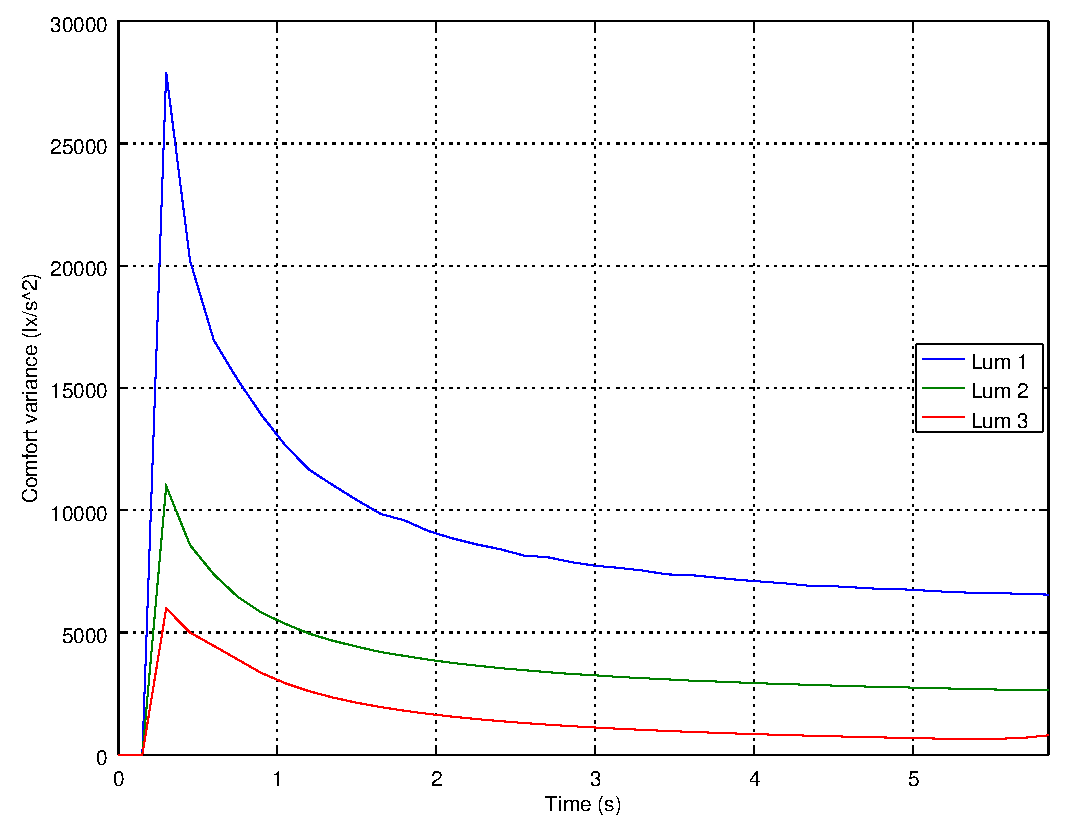
\includegraphics[width=.95\textwidth]{img/f_open_o101}
    \caption{Comfort variance over time of the 3 luminaires.}
    \label{fig:f_open_o101}
    \end{subfigure}
    \begin{subfigure}[t]{0.32\textwidth}
    \centering
    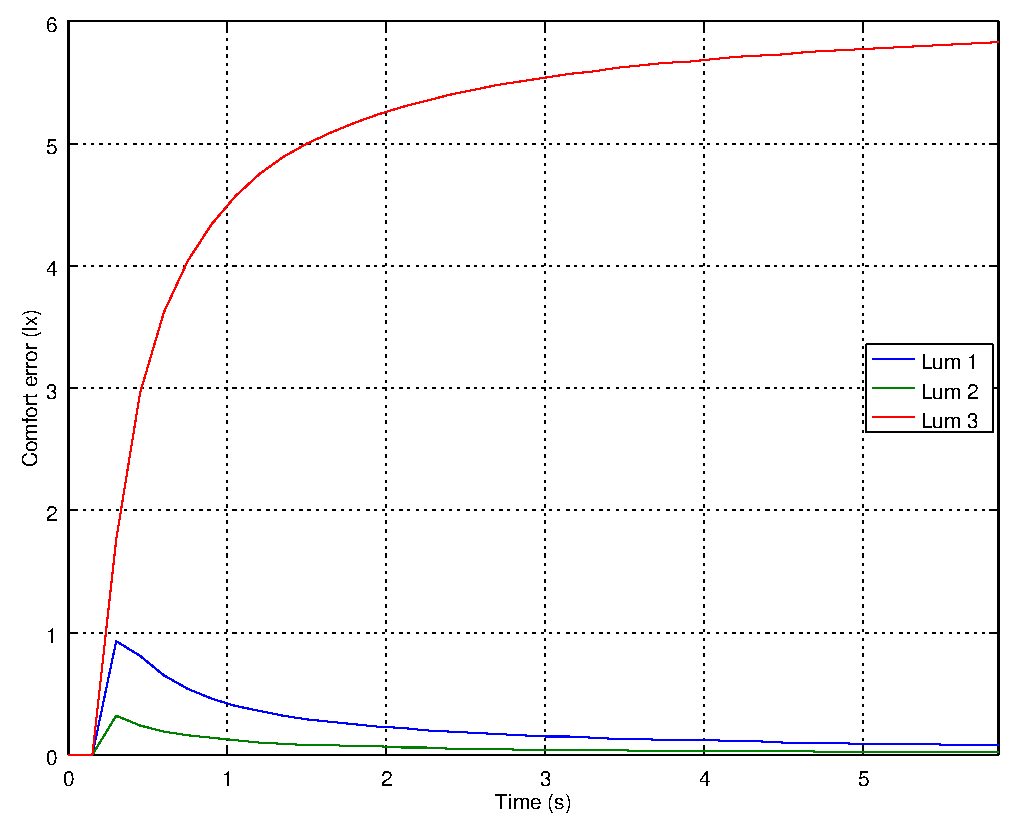
\includegraphics[width=.95\textwidth]{img/n_open_o101}
    \caption{Comfort error over time of the 3 luminaires.}
    \label{fig:n_open_o101}
    \end{subfigure}
    \caption{Metrics after system startup with the box open and desks 1 and 3 as occupied.}
    \label{fig:open_o101}
\end{figure}

%na justificação do conforto do 3 podes dizer que o steady state que mostra que conseguimos chegar até 50 luz foi tirado para o 1
%e o 3 para além de lhe faltar um bocado de papel por baixo é o unico que o LDR nao recebe luz directa do lado direito
%E dizer que a iluminação está lá (até está demais) o sensor é que não a apanha

On Figure~\ref{fig:open_o101} we see some similarities on the behaviour of the metrics. The energy for luminaires 1 and 3 rises linearly however energy spent by luminaire 2 is approximillarly 0. This means that the second LED is off and that it isn't necessary to reach the desired illuminance. The main difference in this result is that the confort error for the luminaire 3 doesn't converge to 0, but to 6. This means that the even with the luminaire at it's maximum intensity the sensor can't read the 30 lux value, only 24. This might seem weird, but there are many reasons to explain this. First the steady state plot on Figure~\ref{fig:steady_state} was taken for luminaire 1 and not 3 that might have different characteristics such as the reflection of the light. Also the 3rd LDR is the only one that doesn't have a LED to it's right. The most important factor is the fact that the box is slightly open, this causes the LED and the LDR to not be directly in their reflection path. 


%\subsection{Energy}
%\subsection{Comfort Error}
%\subsection{Comfort Variance}
